\documentclass[12pt,a4paper]{article}

\usepackage[T1]{fontenc}
\usepackage[utf8]{inputenc}
\usepackage[margin=2cm,headheight=15pt]{geometry}
\usepackage{graphicx}
\usepackage{float}
\usepackage{xcolor}
\usepackage{listings}
\usepackage{fancyhdr}
\usepackage{amsmath}
\usepackage{hyperref}

\graphicspath{{images/}}
\pagestyle{fancy}
\fancyhf{}
\fancyhead[L]{Lab 04 -- Cooperative Scheduler}
\fancyhead[R]{MPU \& MCU}
\fancyfoot[C]{\thepage}
\renewcommand{\headrulewidth}{0.4pt}
\renewcommand{\footrulewidth}{0pt}

\lstset{
    language=C,
    basicstyle=\ttfamily\scriptsize,
    keywordstyle=\color{blue},
    commentstyle=\color{gray},
    stringstyle=\color{red},
    numbers=left,
    numberstyle=\tiny\color{gray},
    numbersep=5pt,
    frame=single,
    breaklines=true,
    keepspaces=true,
    columns=fullflexible,
    showstringspaces=false,
    tabsize=2,
    captionpos=b
}

\begin{document}

\begin{center}
    {\Large\bfseries LAB 04: COOPERATIVE SCHEDULER}\\[4pt]
    {\normalsize Subject: Microprocessor -- Microcontroller (CO2014) \quad | \quad Platform: STM32F103C8 / Proteus 8}
\end{center}
\vspace{-6pt}
\hrule
\vspace{10pt}

\section{Hardware Configuration and Circuit Schematic}

TIM2 generates interrupts every 10~ms using the 8~MHz internal clock (HSI):
\[
T = \frac{(\text{PSC} + 1) \times (\text{ARR} + 1)}{f_{\text{CLK}}} = \frac{(79 + 1) \times (999 + 1)}{8\,000\,000\ \text{Hz}} = 10\ \text{ms}.
\]

\begin{table}[H]
\centering
\small
\begin{tabular}{|l|l|l|l|}
\hline
\textbf{Signal} & \textbf{Pin} & \textbf{Mode} & \textbf{Function} \\ \hline
LED1 -- LED5 & PA0 -- PA4 & Output Push-Pull & 5 periodic task indicators (0.5s, 1.0s, 1.5s, 2.0s, 2.5s) \\ \hline
USART1\_TX / RX & PA9 / PA10 & Alternate Function / Input & Virtual Terminal communication (115200 bps, 8N1) \\ \hline
\end{tabular}
\end{table}

\begin{figure}[H]
    \centering
    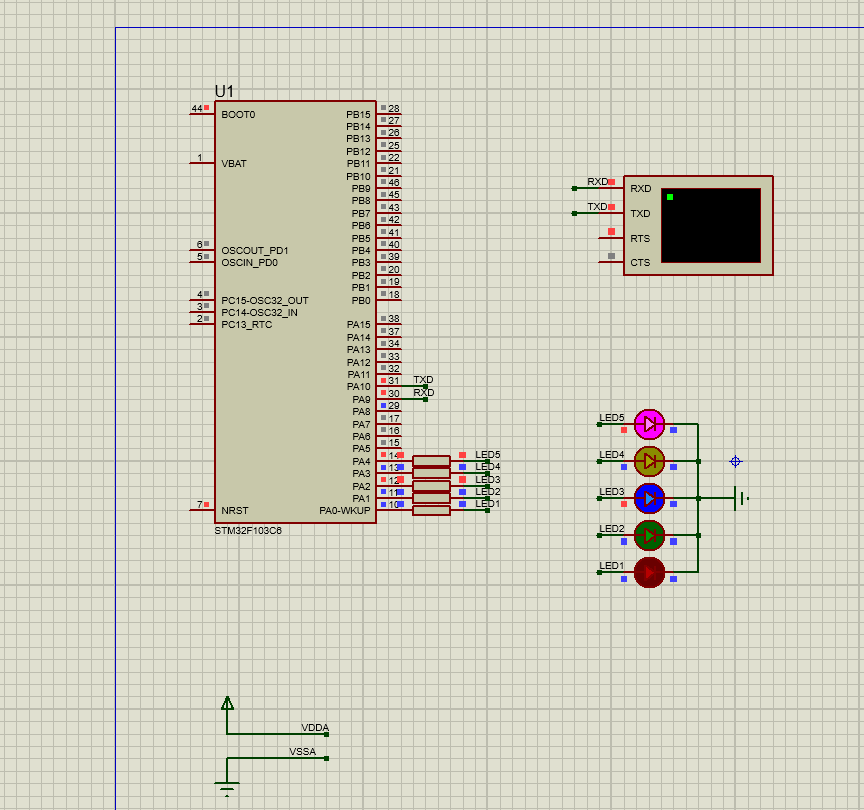
\includegraphics[width=0.88\textwidth,height=0.42\textheight,keepaspectratio]{schematic_crop.png}
    \caption{Proteus schematic: STM32F103, 5 LEDs, and Virtual Terminal}
    \label{fig:schematic}
\end{figure}

\section{Cooperative Scheduler Implementation}

The scheduler maintains a sorted Delta-Time queue. The timer ISR \texttt{SCH\_Update} operates in strictly \textbf{$O(1)$ constant time} by servicing only the task at the head of the queue (\texttt{index = 0}). Critical sections are protected by \texttt{\_\_disable\_irq()} and \texttt{\_\_enable\_irq()}.

\begin{lstlisting}[caption={\texttt{scheduler.h}}]
#ifndef INC_SCHEDULER_H_
#define INC_SCHEDULER_H_
#include "main.h"

#define SCH_MAX_TASKS 10

typedef struct {
    void (*pTask)(void);
    uint32_t Delay;
    uint32_t Period;
    uint8_t RunMe;
    uint32_t TaskID;
} sTask;

void SCH_Init(void);
void SCH_Update(void);
void SCH_Dispatch_Tasks(void);
uint32_t SCH_Add_Task(void (*pFunction)(void), uint32_t DELAY, uint32_t PERIOD);
uint8_t SCH_Delete_Task(uint32_t taskID);
#endif
\end{lstlisting}

\newpage

\begin{lstlisting}[caption={\texttt{scheduler.c}}]
#include "scheduler.h"

static sTask SCH_tasks_G[SCH_MAX_TASKS];
static uint32_t current_task_id = 1;

void SCH_Init(void) {
    for (uint8_t i = 0; i < SCH_MAX_TASKS; i++) {
        SCH_tasks_G[i].pTask = 0;
        SCH_tasks_G[i].Delay = 0;
        SCH_tasks_G[i].Period = 0;
        SCH_tasks_G[i].RunMe = 0;
        SCH_tasks_G[i].TaskID = 0;
    }
}

void SCH_Update(void) {
    if (SCH_tasks_G[0].pTask != 0) {
        if (SCH_tasks_G[0].Delay > 0) SCH_tasks_G[0].Delay--;
        if (SCH_tasks_G[0].Delay == 0) SCH_tasks_G[0].RunMe = 1;
    }
}

uint32_t SCH_Add_Task(void (*pFunction)(void), uint32_t DELAY, uint32_t PERIOD) {
    if (pFunction == 0) return 0;
    __disable_irq();
    uint8_t index = 0;
    while (index < SCH_MAX_TASKS && SCH_tasks_G[index].pTask != 0) {
        if (DELAY < SCH_tasks_G[index].Delay) {
            SCH_tasks_G[index].Delay -= DELAY;
            break;
        } else {
            DELAY -= SCH_tasks_G[index].Delay;
            index++;
        }
    }
    if (index == SCH_MAX_TASKS) {
        __enable_irq();
        return 0;
    }
    for (int8_t i = SCH_MAX_TASKS - 1; i > index; i--) {
        SCH_tasks_G[i] = SCH_tasks_G[i - 1];
    }
    SCH_tasks_G[index].pTask = pFunction;
    SCH_tasks_G[index].Delay = DELAY;
    SCH_tasks_G[index].Period = PERIOD;
    SCH_tasks_G[index].RunMe = (DELAY == 0) ? 1 : 0;
    SCH_tasks_G[index].TaskID = current_task_id++;
    __enable_irq();
    return SCH_tasks_G[index].TaskID;
}

uint8_t SCH_Delete_Task(uint32_t taskID) {
    if (taskID == 0) return 0;
    __disable_irq();
    for (uint8_t i = 0; i < SCH_MAX_TASKS; i++) {
        if (SCH_tasks_G[i].TaskID == taskID) {
            if (i + 1 < SCH_MAX_TASKS && SCH_tasks_G[i + 1].pTask != 0) {
                SCH_tasks_G[i + 1].Delay += SCH_tasks_G[i].Delay;
            }
            for (uint8_t j = i; j < SCH_MAX_TASKS - 1; j++) {
                SCH_tasks_G[j] = SCH_tasks_G[j + 1];
            }
            SCH_tasks_G[SCH_MAX_TASKS - 1].pTask = 0;
            SCH_tasks_G[SCH_MAX_TASKS - 1].Delay = 0;
            SCH_tasks_G[SCH_MAX_TASKS - 1].Period = 0;
            SCH_tasks_G[SCH_MAX_TASKS - 1].RunMe = 0;
            SCH_tasks_G[SCH_MAX_TASKS - 1].TaskID = 0;
            __enable_irq();
            return 1;
        }
    }
    __enable_irq();
    return 0;
}

void SCH_Dispatch_Tasks(void) {
    while (SCH_tasks_G[0].pTask != 0 && (SCH_tasks_G[0].RunMe > 0 || SCH_tasks_G[0].Delay == 0)) {
        void (*pFunction)(void) = SCH_tasks_G[0].pTask;
        uint32_t period = SCH_tasks_G[0].Period;
        (*pFunction)();
        SCH_Delete_Task(SCH_tasks_G[0].TaskID);
        if (period > 0) {
            SCH_Add_Task(pFunction, period, period);
        }
    }
}
\end{lstlisting}

\newpage

\section{Application Tasks and Main Loop (\texttt{main.c})}

Standard \texttt{printf} is redirected to USART1 via \texttt{\_write}. Five periodic tasks are registered with their respective periods in 10~ms ticks (50, 100, 150, 200, 250).

\begin{lstlisting}[caption={Application tasks and main loop in \texttt{main.c}}]
int _write(int file, char *ptr, int len) {
    HAL_UART_Transmit(&huart1, (uint8_t*)ptr, len, 50);
    return len;
}

void Task1_LED1(void) {
    HAL_GPIO_TogglePin(GPIOA, LED1_Pin);
    printf("[%lu ms] Task 1 (0.5s)\r\n", HAL_GetTick());
}
void Task2_LED2(void) {
    HAL_GPIO_TogglePin(GPIOA, LED2_Pin);
    printf("[%lu ms] Task 2 (1.0s)\r\n", HAL_GetTick());
}
void Task3_LED3(void) {
    HAL_GPIO_TogglePin(GPIOA, LED3_Pin);
    printf("[%lu ms] Task 3 (1.5s)\r\n", HAL_GetTick());
}
void Task4_LED4(void) {
    HAL_GPIO_TogglePin(GPIOA, LED4_Pin);
    printf("[%lu ms] Task 4 (2.0s)\r\n", HAL_GetTick());
}
void Task5_LED5(void) {
    HAL_GPIO_TogglePin(GPIOA, LED5_Pin);
    printf("[%lu ms] Task 5 (2.5s)\r\n", HAL_GetTick());
}

void HAL_TIM_PeriodElapsedCallback(TIM_HandleTypeDef *htim) {
    if (htim->Instance == TIM2) SCH_Update();
}

int main(void) {
    HAL_Init();
    SystemClock_Config();
    MX_GPIO_Init();
    MX_TIM2_Init();
    MX_USART1_UART_Init();

    HAL_TIM_Base_Start_IT(&htim2);
    SCH_Init();

    SCH_Add_Task(Task1_LED1, 50, 50);    // 500 ms = 50 ticks
    SCH_Add_Task(Task2_LED2, 100, 100);  // 1000 ms = 100 ticks
    SCH_Add_Task(Task3_LED3, 150, 150);  // 1500 ms = 150 ticks
    SCH_Add_Task(Task4_LED4, 200, 200);  // 2000 ms = 200 ticks
    SCH_Add_Task(Task5_LED5, 250, 250);  // 2500 ms = 250 ticks

    while (1) {
        SCH_Dispatch_Tasks();
    }
}
\end{lstlisting}

\newpage

\section{Simulation Results and Demonstration Verification}

Figure~\ref{fig:terminal} displays the real-time execution log captured from the Proteus Virtual Terminal.

\begin{figure}[H]
    \centering
    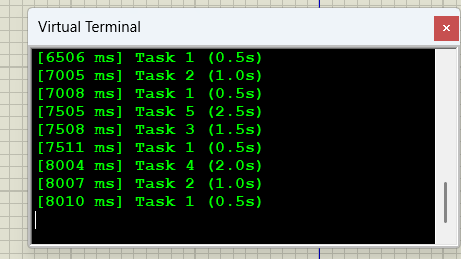
\includegraphics[width=0.68\textwidth,keepaspectratio]{terminal_crop.png}
    \caption{Captured execution timestamps on Proteus Virtual Terminal}
    \label{fig:terminal}
\end{figure}

\begin{table}[H]
\centering
\small
\begin{tabular}{|c|c|l|c|}
\hline
\textbf{Expected Deadline} & \textbf{Actual Timestamp} & \textbf{Executed Task} & \textbf{Error / Jitter} \\ \hline
6500 ms & 6506 ms & Task 1 (0.5s) & $+6$ ms \\ \hline
7000 ms & 7005 ms & Task 2 (1.0s) & $+5$ ms \\ 
        & 7008 ms & Task 1 (0.5s) & $+8$ ms \\ \hline
7500 ms & 7505 ms & Task 5 (2.5s) & $+5$ ms \\ 
        & 7508 ms & Task 3 (1.5s) & $+8$ ms \\ 
        & 7511 ms & Task 1 (0.5s) & $+11$ ms \\ \hline
8000 ms & 8004 ms & Task 4 (2.0s) & $+4$ ms \\ 
        & 8007 ms & Task 2 (1.0s) & $+7$ ms \\ 
        & 8010 ms & Task 1 (0.5s) & $+10$ ms \\ \hline
\end{tabular}
\caption{Timing accuracy and multi-task collision resolution}
\label{tab:results}
\end{table}

\textbf{Analysis:}
\begin{enumerate}
    \item \textbf{Timing Accuracy:} Every task executes within $\pm 10$~ms of its scheduled deadline.
    \item \textbf{Collision Resolution:} At $t = 7500$~ms (shared deadline for Tasks 1, 3, and 5) and $t = 8000$~ms (Tasks 1, 2, and 4), the dispatcher executes each ready task sequentially without starvation or dropped events. The $\sim 3$~ms interval between consecutive tasks reflects the non-blocking UART character transmission in user mode.
    \item \textbf{Satisfying Lab Criteria:}
    \begin{itemize}
        \item Multiple concurrent timeouts supported.
        \item Callbacks delivered in strict chronological order.
        \item Elimination of $O(n)$ search in \texttt{SCH\_Update} ($O(1)$ head-only execution).
        \item Clean 10~ms timer tick operation.
    \end{itemize}
\end{enumerate}

\end{document}
